\begin{figure}[htbp]
\section*{ ATP6V0C}
\centering
\begin{subfigure}[b]{0.95\textwidth}
\centering
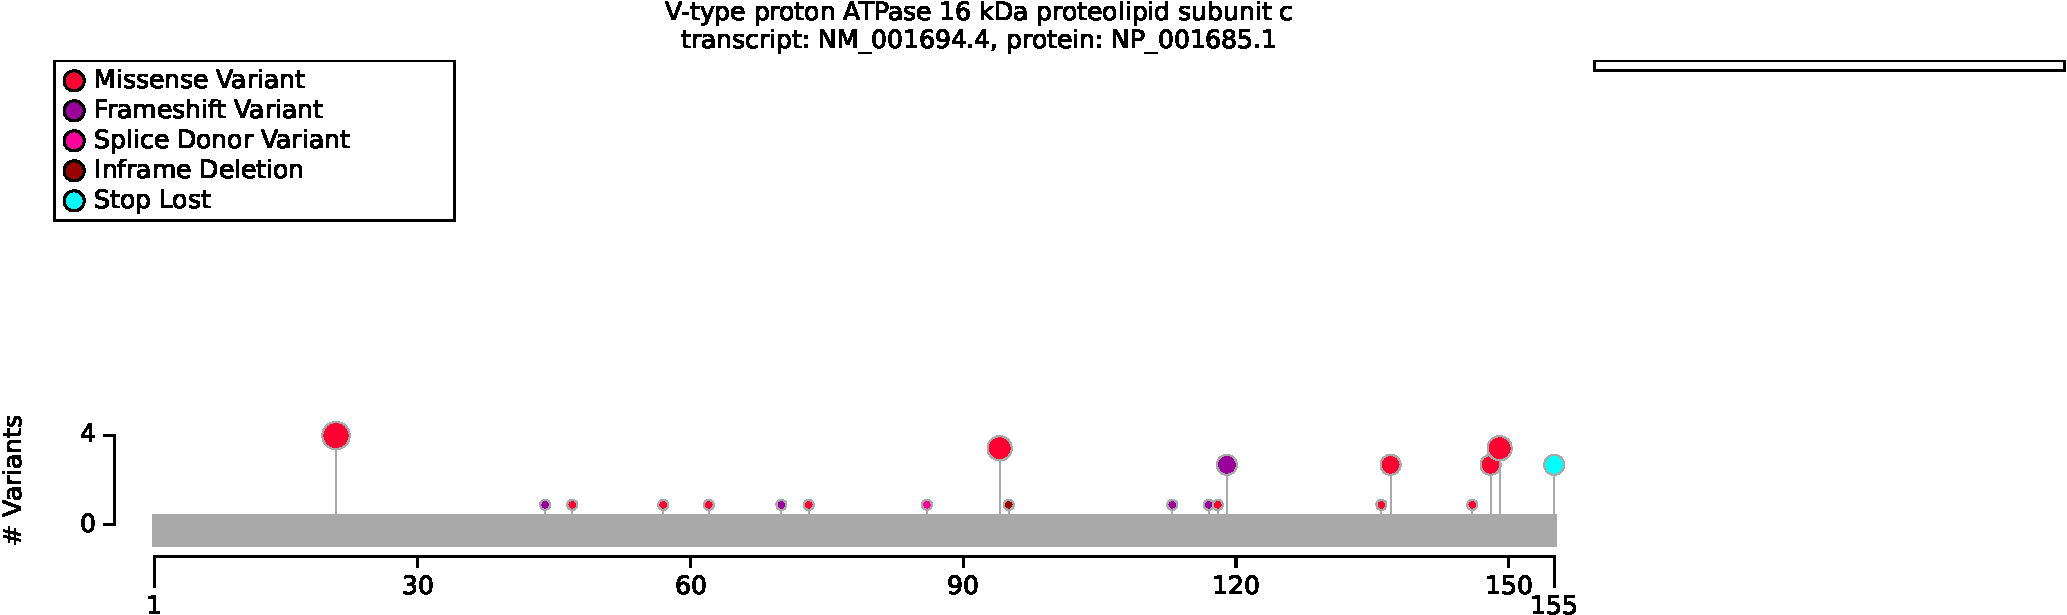
\includegraphics[width=\textwidth]{ img/ATP6V0C_protein_diagram.pdf} 
\captionsetup{justification=raggedright,singlelinecheck=false}
\caption{Distribution of variants in ATP6V0C}
\end{subfigure}

\vspace{2em}

\begin{subfigure}[b]{0.95\textwidth}
\centering
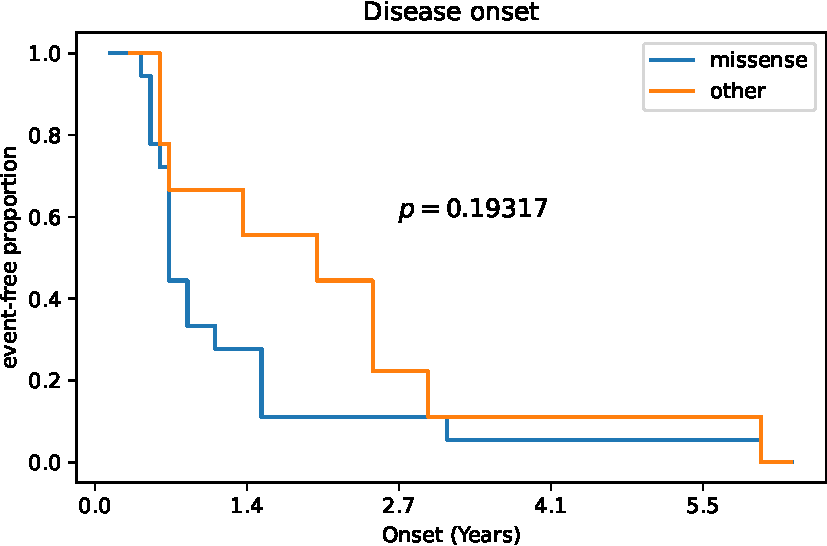
\includegraphics[width=0.3\textwidth]{ img/ATP6V0C_stats.pdf} 
\captionsetup{justification=raggedright,singlelinecheck=false}
\caption{Disease onset for  ATP6V0C missense vs. other variants.}
\end{subfigure}

\vspace{2em}

\begin{subfigure}[b]{0.95\textwidth}
\centering
\resizebox{\textwidth}{!}{
\begin{tabular}{llllrr}
\toprule
Genotype (A) & Genotype (B) & total tests performed & significant results\\
\midrule
1-100 & 100+ & 80 & 0\\
missense & other & 80 & 0\\
FEMALE & MALE & 80 & 0\\
\bottomrule
\end{tabular}
}
\captionsetup{justification=raggedright,singlelinecheck=false}
\caption{Fisher Exact Test performed to compare HPO annotation frequency with respect to genotypes. }
\end{subfigure}

\vspace{2em}

\begin{subfigure}[b]{0.95\textwidth}
\captionsetup{justification=raggedright,singlelinecheck=false}
\resizebox{\textwidth}{!}{
\begin{tabular}{llllrr}
\toprule
Description & Variable & Genotype (A) & Genotype (B) & p-value & xrefs\\
\midrule
Compute time until OMIM:620465 onset & Onset of OMIM:620465 & missense & other & 0.193 & -\\
\bottomrule
\end{tabular}
}
\caption{ Onset of OMIM:620465 to compare missense and other with respect to Onset of OMIM:620465. }
\end{subfigure}

\vspace{2em}

\caption{ The cohort comprised 31 individuals (12 females, 19 males). A total of 83 HPO terms were used to annotate the cohort. Disease diagnosis: Epilepsy, early-onset, 3, with or without developmental delay (OMIM:620465). to do. A total of 23 unique variant alleles were found in \textit{ATP6V0C} (transcript: \texttt{NM\_001694.4}, protein id: \texttt{NP\_001685.1}).}
\end{figure}
